\documentclass[handout]{beamer}
\mode<presentation>{}
\usetheme{Montpellier}
\usecolortheme{dolphin}
\usepackage{apalike}
\usepackage{graphicx}
\usepackage{subcaption}
\usepackage{pgfplotstable}
\usepackage{ amssymb }
\usepackage{graphicx,psfrag}
\usepackage{subcaption}
\usepackage{mwe,tikz}\usepackage[percent]{overpic}
%% preamble
\title{Robust Computational Models for Water Waves}
\author{Jordan Pitt, Stephen Roberts and Christopher Zoppou \\ Australian National University}
\newcommand\solidrule[1][0.25cm]{\rule[0.5ex]{#1}{1pt}}
\newcommand\dashedrule{\mbox{\solidrule[2mm]\hspace{2mm}\solidrule[2mm]}}
\newcommand{\dotrule}[1]{%
	\parbox[]{#1}{\dotfill}}

\setbeamertemplate{navigation symbols}{}

\newcommand\blfootnote[1]{%
	\begingroup
	\renewcommand\thefootnote{}\footnote{#1}%
	\addtocounter{footnote}{-1}%
	\endgroup
}


\begin{document}
	\begin{frame}<presentation:0>
		\cite{Zoppou-2014} \cite{Pitt-2018-61}
	\end{frame}
%% title frame
\begin{frame}
\titlepage
\end{frame}
\begin{frame}{Outline of the Presentation}
	%Modelling Process
	%SWWE
	%Serre
	%My Work
	
	\begin{itemize}
		\item Motivation
		\item History
		\item Contribution 
		\begin{itemize}
			\item Method
			\item Validation
		\end{itemize}
	\end{itemize}
	
\end{frame}

\section{Water Wave Modelling}
\subsection{Introduction}

\begin{frame}{Physical Phenomena: Water Waves}
	Water wave hazards:
	\begin{itemize}
		\item Tsunamis
		\item Storm Surges
		\item Rogue Waves
	\end{itemize}
	\smallskip
	\pause
	Phenomena caused by water waves:
	\begin{itemize}
		\item Nutrient Transport
		\item Beach Erosion
		\item Breakup of Sea Ice
	\end{itemize}
\end{frame}
%Cool pictures


\begin{frame}{Computational Modelling}
	%Picture Physical Process -> Mathematical Description -> Studying Mathematical Description (Numerical Solution)
	Goal: Model Physics On Computers \pause
	\begin{figure}
		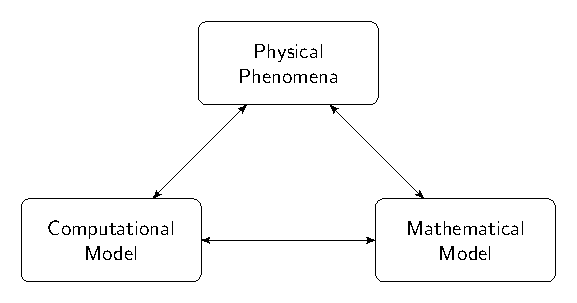
\includegraphics[width=\textwidth]{./Pics/ModelDiagrams/FlowChart.pdf}
	\end{figure}
\end{frame}

\begin{frame}{ANUGA}
	\begin{figure}
		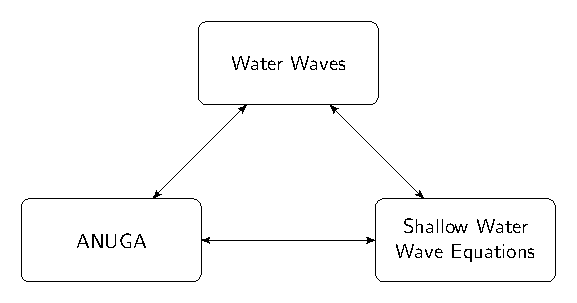
\includegraphics[width=\textwidth]{./Pics/ModelDiagrams/FlowChartANUGA.pdf}
	\end{figure}
\end{frame}

\begin{frame}{ANUGA: Water Waves}
	\begin{figure}
		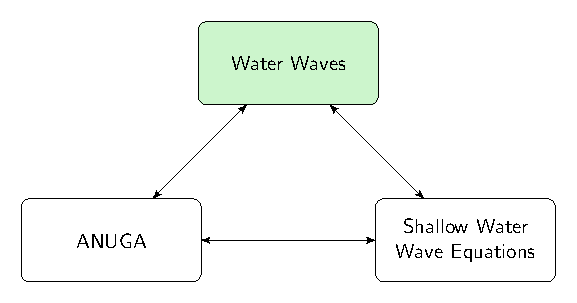
\includegraphics[width=\textwidth]{./Pics/ModelDiagrams/FlowChartANUGA1G.pdf}
	\end{figure}
	%main physical drivers
\end{frame}

\begin{frame}{ANUGA: Shallow Water Wave Equations}
	\begin{figure}
		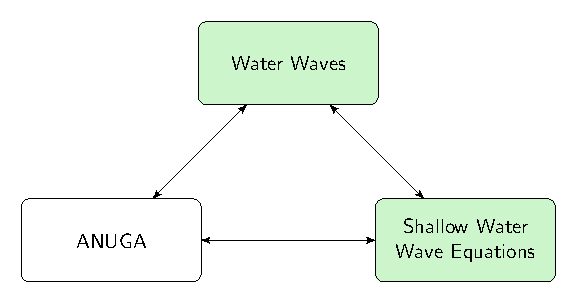
\includegraphics[width=\textwidth]{./Pics/ModelDiagrams/FlowChartANUGA12G.pdf}
	\end{figure}
	%main physical drivers it captures: nonlinearity and bed effects
\end{frame}

\begin{frame}{ANUGA}
	\begin{figure}
		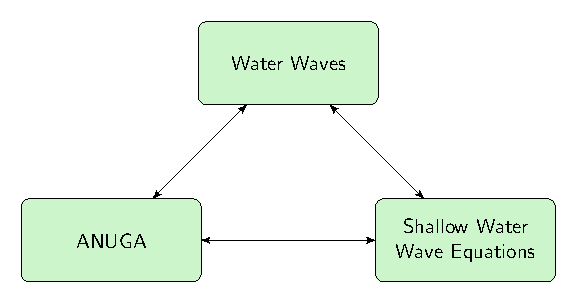
\includegraphics[width=\textwidth]{./Pics/ModelDiagrams/FlowChartANUGA123G.pdf}
	\end{figure}
\end{frame}


\begin{frame}{Outcome}
 New project at the ANU to build robust computational model from dispersive mathematical models
\end{frame}
%mention previous work of ANU

\subsection{Serre Model}


\subsection{Serre Model}
\begin{frame}{Mathematical Model}
	%Picture Physical Process -> Mathematical Description -> Studying Mathematical Description (Numerical Solution)
	\begin{figure}
		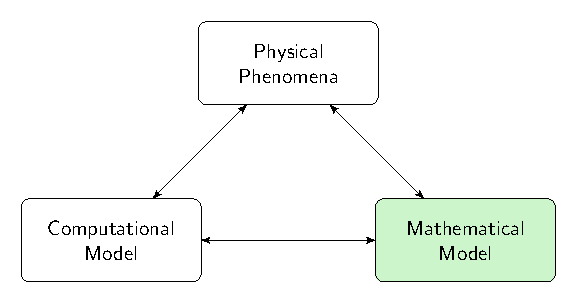
\includegraphics[width=\textwidth]{./Pics/ModelDiagrams/FlowChartHigh2G.pdf}
	\end{figure}
\end{frame}
\begin{frame}{Serre Model}
	\begin{figure}
		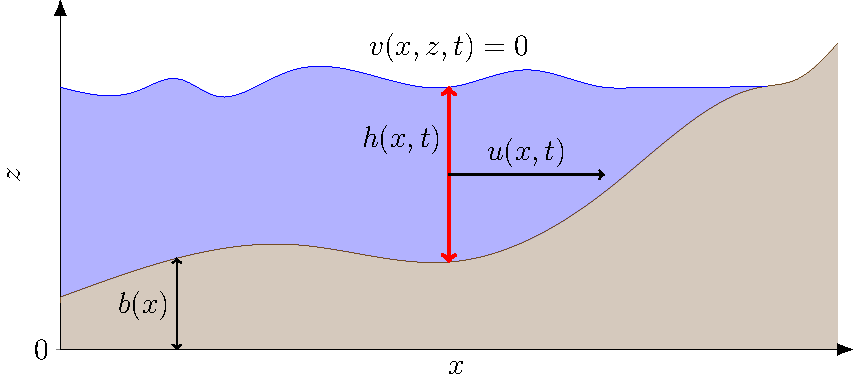
\includegraphics[width=\textwidth]{./Pics/WaterModelDiagrams/SWWE.pdf}
	\end{figure}
\end{frame}
\begin{frame}{Assumptions}
	\begin{itemize}
		\pause
		\item Particle: $u'(x,z,t)$ constant in $z$
		\pause
		\item Particle: $v'(x,z,t) = u\frac{\partial b}{\partial x} - (z - b)\frac{\partial b}{\partial x}$
		\pause
		\item Particle: $p'(x,z,t) = g\xi  + \xi { \color{red}\Psi } + \frac{1}{2} \xi \left(2h - \xi\right) { \color{blue} \Phi }$
	\end{itemize}
		with
		\begin{align*}
		&{ \color{red}\Psi }  = \dfrac{\partial b}{\partial x}\left(\dfrac{\partial u}{\partial t} + u\dfrac{\partial u}{\partial x} \right)  + u^2\dfrac{\partial^2 b}{\partial x^2}, \\&
		{ \color{blue} \Phi }  = \dfrac{\partial u }{\partial x} \dfrac{\partial u}{\partial x} -u \dfrac{\partial^2 u}{\partial x^2}  - \dfrac{\partial^2 u}{\partial x \partial t} .
		\end{align*}
\end{frame}
\begin{frame}{Equations}
	\begin{subequations}
		\begin{align*}
		&\text{Mass:} && \frac{\partial h}{\partial t} + \dfrac{\partial (uh)}{\partial x} = 0,  \\ \\
		&\text{Momentum:} &&\dfrac{\partial (uh)}{\partial t} + \dfrac{\partial}{\partial x} \left ( u^2h + \dfrac{gh^2}{2} + \dfrac{h^2}{2}{ \color{red}\Psi } + \dfrac{h^3}{3}{ { \color{blue} \Phi } }  \right )   \\ \\& &&\quad \quad \; \; +  \dfrac{\partial b}{\partial x} \left (gh +   h { \color{red}\Psi } + \dfrac{h^2}{2}{ { \color{blue} \Phi } }  \right ) = 0.
		\end{align*}
	\end{subequations}
		\begin{align*}
		&{ \color{red}\Psi }  = \dfrac{\partial b}{\partial x}\left(\dfrac{\partial u}{\partial t} + u\dfrac{\partial u}{\partial x} \right)  + u^2\dfrac{\partial^2 b}{\partial x^2}, &
		{ \color{blue} \Phi }  = \dfrac{\partial u }{\partial x} \dfrac{\partial u}{\partial x} -u \dfrac{\partial^2 u}{\partial x^2}  - \dfrac{\partial^2 u}{\partial x \partial t} .
		\end{align*}
\end{frame}
\begin{frame}{Pros and Cons}
	Pro:
	\begin{itemize}
		\item Far simpler than the Euler equations
		\item Includes dispersive effects
		\item Still a good model for long wavelength waves and also a good model for shorter wavelengths
		\item Considered one of the best models for water waves up to wave breaking
	\end{itemize}
	Cons:
	\begin{itemize}
		\item More complicated than the Shallow Water Wave Equations
		\item Cannot model breaking waves
	\end{itemize}
\end{frame}
\begin{frame}{Computational Model}
	%Picture Physical Process -> Mathematical Description -> Studying Mathematical Description (Numerical Solution)
	\begin{figure}
		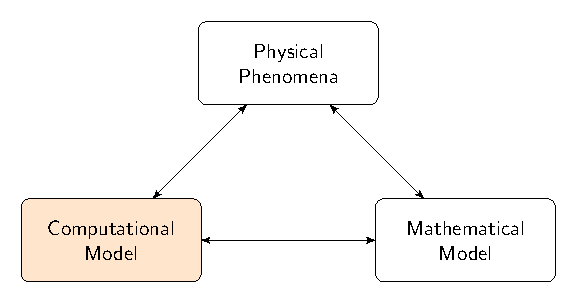
\includegraphics[width=\textwidth]{./Pics/ModelDiagrams/FlowChartHigh3O.pdf}
	\end{figure}
\end{frame}
\begin{frame}{Previous Work at the ANU}
	\begin{itemize}
		\item 2014: Chris Zoppou's PhD thesis  \\
			Demonstrated computational model based on Finite Volume Method for the Serre equations with varying bathymetry in 2D.
		\item 2014: My Honours thesis \\
			Independent reproduction of Chris Zoppou's computational model
	\end{itemize}
	\pause
	Open problems:
	\begin{itemize}
		\item[3D:] Extension of the method to 3D flows
		\item[Robust:] Validation of model with steep gradients in free surface
		\item[Robust:] Validation of model in the presence of dry beds
	\end{itemize}	
\end{frame}



\section{Thesis}
%Goal of thesis to develop numerical method that can handle dry beds and steep gradients using FEM and FVM

\begin{frame}{Thesis Goals}
	Solve these open problems:
	\begin{itemize}
		\item[3D:] Extension of the method to 3D flows
		\item[Robust:] Validation of model with steep gradients in free surface
		\item[Robust:] Validation of model in the presence of dry beds
	\end{itemize}		
	\medskip
	\pause
	Technique: Develop a robust computational model from the 2D Serre equations that can be easily extended to 3D. 
\end{frame}

\begin{frame}{Method}
	Brief description of the method which is a combination of a Finite Volume Method and a Finite Element method. 
\end{frame}
\subsection{Finite Volume Method}
\begin{frame}{Finite Volume Method}
\begin{itemize}
	\item[3D:] Extends well to 3D
	\item[Robust:] Stable in the presence of steep gradients
	\item[Robust:] Stable in the presence of dry beds
	\item Maintains conservation properties of the equations
\end{itemize}
\pause  Chris Zoppou's thesis demonstrated how an adaptation of the Finite Volume Method to the Serre Equations.
\end{frame}

\begin{frame}{Equations}
		\begin{subequations}
			\begin{align*}
			&\frac{\partial h}{\partial t} + \dfrac{\partial (uh)}{\partial x} = 0,  \\ \\
			&\dfrac{\partial (uh)}{\partial t} + \dfrac{\partial}{\partial x} \left ( u^2h + \dfrac{gh^2}{2} + \dfrac{h^2}{2}{ \color{red}\Psi } + \dfrac{h^3}{3}{ { \color{blue} \Phi } }  \right )  +  \dfrac{\partial b}{\partial x} \left (gh +   h { \color{red}\Psi } + \dfrac{h^2}{2}{ { \color{blue} \Phi } }  \right ) = 0
			\end{align*}
		\end{subequations}
				\begin{align*}
				&{ \color{red}\Psi }  = \dfrac{\partial b}{\partial x}\left(\dfrac{\partial u}{\partial t} + u\dfrac{\partial u}{\partial x} \right)  + u^2\dfrac{\partial^2 b}{\partial x^2}, &
				{ \color{blue} \Phi }  = \dfrac{\partial u }{\partial x} \dfrac{\partial u}{\partial x} -u \dfrac{\partial^2 u}{\partial x^2}  - \dfrac{\partial^2 u}{\partial x \partial t} .
				\end{align*}
	\pause
	For a Finite Volume Method we require equations in the form
	\begin{equation*}
	\frac{\partial q}{\partial t} + \frac{\partial f(q)}{\partial x} + s(q) = 0
	\end{equation*}
	where $f(q)$ and $s(q)$ do not contain temporal derivatives
\end{frame}


\begin{frame}{Finite Volume Method Example}
	\begin{equation*}
	\frac{\partial q}{\partial t} + \frac{\partial f(q)}{\partial x} + s(q) = 0
	\end{equation*}	
\end{frame}
\begin{frame}{Function at $t=t_0$}
	\begin{figure}
		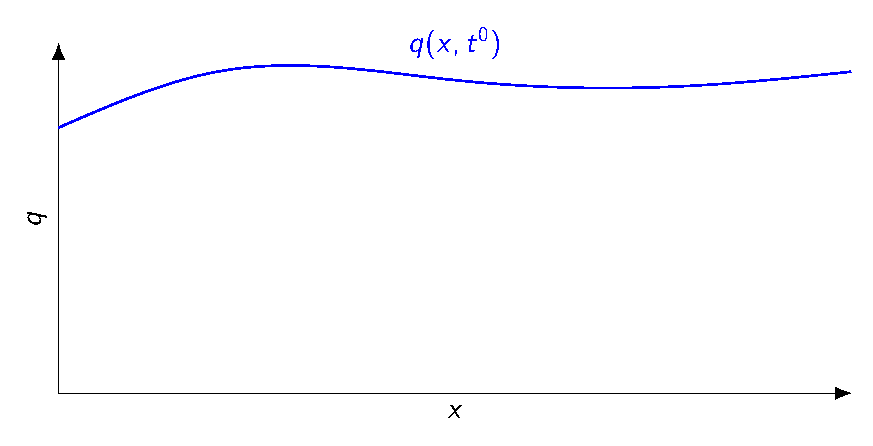
\includegraphics[width=\textwidth]{./Pics/FVMpicture/Function.pdf}
	\end{figure}
\end{frame}
\begin{frame}{Cell Discretisation}
	\begin{figure}
		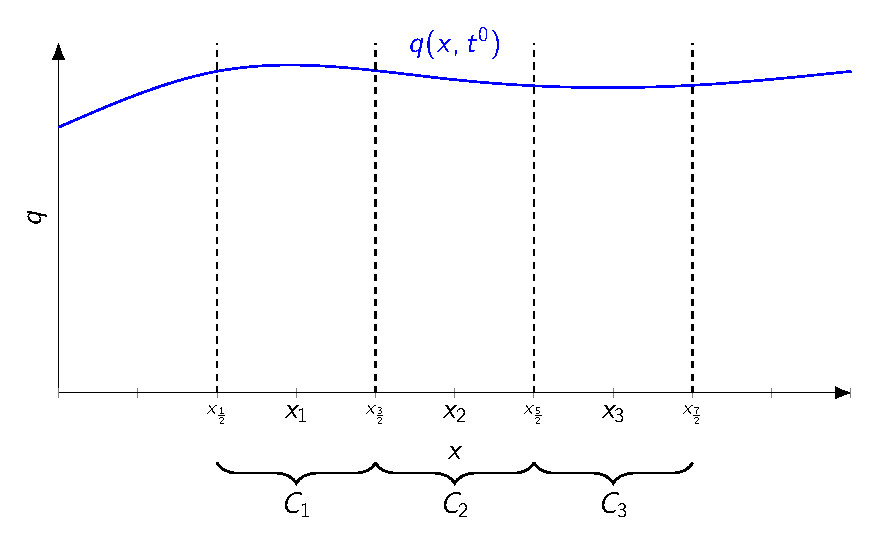
\includegraphics[width=\textwidth]{./Pics/FVMpicture/Cells.pdf}
	\end{figure}
\end{frame}
\begin{frame}{Total Amount}
	\begin{figure}
		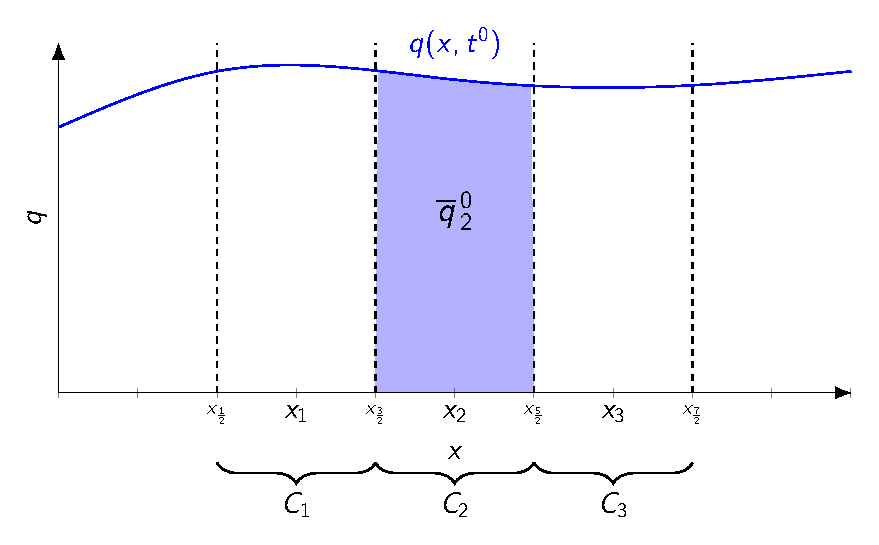
\includegraphics[width=0.9\textwidth]{./Pics/FVMpicture/Total.pdf}
	\end{figure}
\end{frame}
\begin{frame}{Flux Left}
	\begin{figure}
		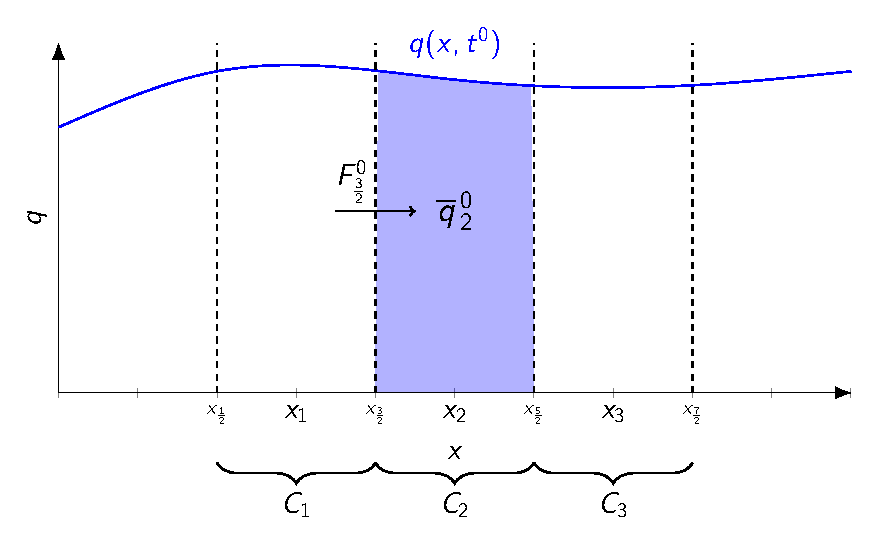
\includegraphics[width=\textwidth]{./Pics/FVMpicture/TotalFluxIn.pdf}
	\end{figure}
\end{frame}
\begin{frame}{Flux Right}
	\begin{figure}
		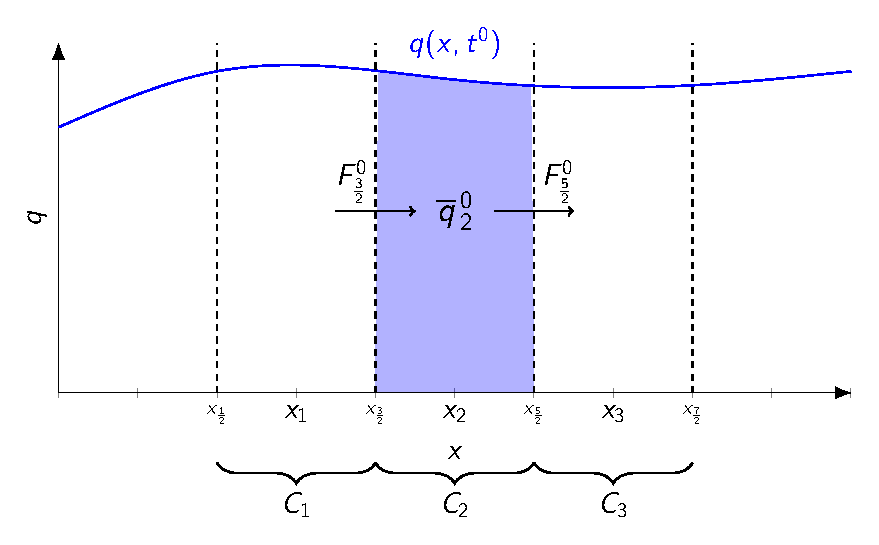
\includegraphics[width=\textwidth]{./Pics/FVMpicture/TotalFluxInOut.pdf}
	\end{figure}
\end{frame}
\begin{frame}{Source}
	\begin{figure}
		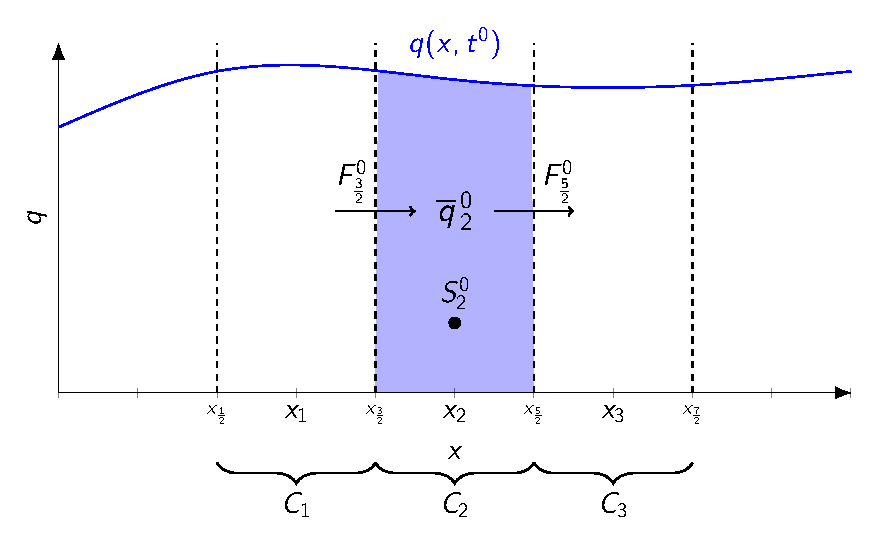
\includegraphics[width=\textwidth]{./Pics/FVMpicture/TotalFluxInOutSource.pdf}
	\end{figure}
\end{frame}
\begin{frame}{Finite Volume Update}
	\begin{equation*}
	\overline{q}^1_2 = \overline{q}^0_2 - \left(F^0_{\frac{5}{2}} - F^0_{\frac{3}{2}}\right) - \left(S^0_2\right)
	\end{equation*}	
	\pause
	\begin{equation*}
	\frac{\partial q}{\partial t} + \frac{\partial f(q)}{\partial x} + s(q) = 0
	\end{equation*}	
\end{frame}
\begin{frame}{Finite Volume Update}	
	\begin{equation*}
	\overline{q}^1_2 = \overline{q}^0_2 - \left(F^0_{\frac{5}{2}} - F^0_{\frac{3}{2}}\right) - \left(S^0_2\right)
	\end{equation*}	
	\begin{equation*}
	{\color{blue}\frac{\partial q}{\partial t}} + {\color{red}\frac{\partial f(q)}{\partial x} } + {\color{green!40!black} s(q) } = 0
	\end{equation*}	
	\pause
	\begin{multline*}
	\overbrace{ {\color{blue}\int_{C_2} q(x,t^1) \; dx}}^{\overline{q}^1_2} = \overbrace{ {\color{blue}\int_{C_2} q(x,t^0) \; dx } }^{\overline{q}^0_2} -  \bigg( \overbrace{ {\color{red}\int_{t^0}^{t^1} f(q(x_{5/2},t)) \; dt}}^{F^0_{\frac{5}{2}}} \\- \overbrace{{\color{red}\int_{t^0}^{t^1} f(q(x_{3/2},t)) \; dt}}^{F^0_{\frac{3}{2}}}  \bigg) -  \overbrace{ {\color{green!40!black}\int_{t^0}^{t^1} \int_{C_2} s(q(x,t)) \; dt }}^{S^0_{2}}
	\end{multline*}
\end{frame}



\begin{frame}{Update Formula for Serre Equations}
	\begin{equation*}
	\overline{h}_j^{n+1} = \overline{h}_j^n -  \left[F_{j + 1/2}^n - F_{j - 1/2}^n \right]
	\end{equation*}
	\begin{equation*}
	\overline{G}_j^{n+1}  = \overline{G}_j^n -  \left[F_{j + 1/2}^n - F_{j - 1/2}^n \right] -  S^n_j
	\end{equation*}
	\pause
	\begin{itemize}
		\item All the fluxes $F^n_{j + 1/2}$ and $F^n_{j - 1/2}$ and the source term $ S^n_j$ require $u$
		\item require a method to obtain $u$ from $\overline{h}^n_j $, $\overline{G}^n_j $ and $b$
	\end{itemize}
	
\end{frame}

\subsection{Finite Element Method}
\begin{frame}{Calculate Velocity}
		\[ G =  h {u} \left(1 + \frac{\partial h}{\partial x}\frac{\partial b}{\partial x} + \frac{1}{2}h\frac{\partial^2 b}{\partial x^2} + \left[\frac{\partial b}{\partial x}\right]^2 \right) - \frac{\partial}{\partial x}\left(\frac{1}{3}h^3  \frac{\partial {u}}{\partial x}\right).\]
		\pause
		\begin{itemize}
			\item Chris Zoppou's Thesis used a Finite Difference Method
			\item Goal: Solve using a Finite Element Method
		\end{itemize}
\end{frame}

\begin{frame}{Finite Element Method}
	\begin{itemize}
		\item[3D:] Extends well to 3D
		\item[Robust:] Stable in the presence of steep gradients 
		\item Maintains conservation properties for conservation equations
	\end{itemize}
\end{frame}

\begin{frame}{Finite Element Method Example}
	Example:
		\[  -\frac{\partial^2 {u}}{\partial x^2}= f.\]
	Weak Form
	\[
	 -\int_{\Omega }\frac{\partial^2 {u}}{\partial x^2} v = \int_{\Omega } f v \; dx
	\]
	Integrate by parts (Dirichlet boundary conditions):
	\[
  \int_{\Omega }\frac{\partial {u}}{\partial x} \frac{\partial {v}}{\partial x} \; dx  = \int_{\Omega } f v \; dx
	\]
\end{frame}

\begin{frame}{Finite Element Method}
	\[
	 \int_{\Omega }\frac{\partial {u}}{\partial x} \frac{\partial {v}}{\partial x} \; dx  = \int_{\Omega } f v \; dx
	\]
	\[
	 \sum_j  \left[\int_{C_j} \frac{\partial {u}}{\partial x} \frac{\partial {v}}{\partial x} \; dx \right] = \sum_j \left[ \int_{C_j} f v  \; dx \right]
	\]

\end{frame}
\begin{frame}{Piecewise Polynomial Representation}
	\begin{figure}
		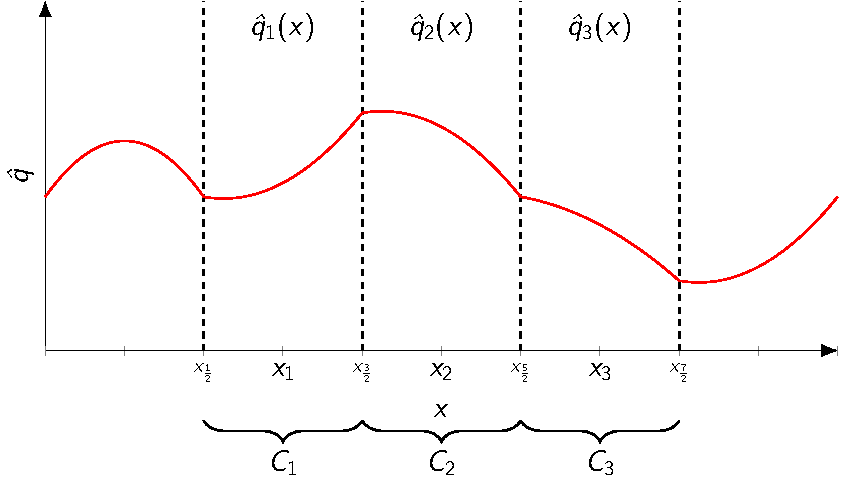
\includegraphics[width=\textwidth]{./Pics/PolyRep/P2.pdf}
	\end{figure}
\end{frame}


\begin{frame}{Finite Element Method}
	\[
	  \sum_j  \left[\int_{C_j} \frac{\partial {u_j }}{\partial x} \frac{\partial {v_j }}{\partial x} \; dx\right]  = \sum_j \left[ \int_{C_j} f_j v_j  \; dx \right]
	\]
	\begin{equation*}
	\boldsymbol{A} \vec{u} = \vec{c}
	\end{equation*}
	where 
	\begin{itemize}
		\item $\boldsymbol{A}$ depends on the polynomial representation of $v$
		\item $\vec{u}$ determines the polynomial representation of $u$
		\item $\vec{c}$ depends on polynomial representation of $f$ and $v$
	\end{itemize}
\end{frame}

\begin{frame}{Finite Element Method for Serre Equations}
		\[ G =  h {u} \left(1 + \frac{\partial h}{\partial x}\frac{\partial b}{\partial x} + \frac{1}{2}h\frac{\partial^2 b}{\partial x^2} + \left[\frac{\partial b}{\partial x}\right]^2 \right) - \frac{\partial}{\partial x}\left(\frac{1}{3}h^3  \frac{\partial {u}}{\partial x}\right).\]
	\pause
	\begin{equation*}
	\boldsymbol{A} \vec{u} = \vec{c}
	\end{equation*}
	where 
	\begin{itemize}
		\item $\boldsymbol{A}$ depends on the polynomial representation of $h$, $b$ and test function
		\item $\vec{u}$ determines the polynomial representation of $u$
		\item $\vec{c}$ depends on polynomial representation of $G$ and test function
	\end{itemize}
\end{frame}


\begin{frame}{Method}
	\begin{itemize}
		\item Reconstruction: Calculate the representations of $h$ and $G$ over the cells from the averages $\bar{h}$ and $\bar{G}$
		\item Finite Element: use the representations of $h$ and $G$ over the cells to calculate the representation of $u$ over the cell
		\item Finite Volume Method: Update $h$ and $G$ to the next time using the Finite Volume Method update
	\end{itemize}
\end{frame}

\begin{frame}{Progress}
	\begin{itemize}
		\item[3D:] Extension of the method to 3D flows  \checkmark
		\item[Robust:] Validation of model with steep gradients in free surface
		\item[Robust:] Validation of model in the presence of dry beds
	\end{itemize}
\end{frame}



\subsection{ Model Validation for Steep Gradients in the Flow}
\begin{frame}{Statement of Problem}
	How does this initially still body of water evolve?
	\begin{figure}
		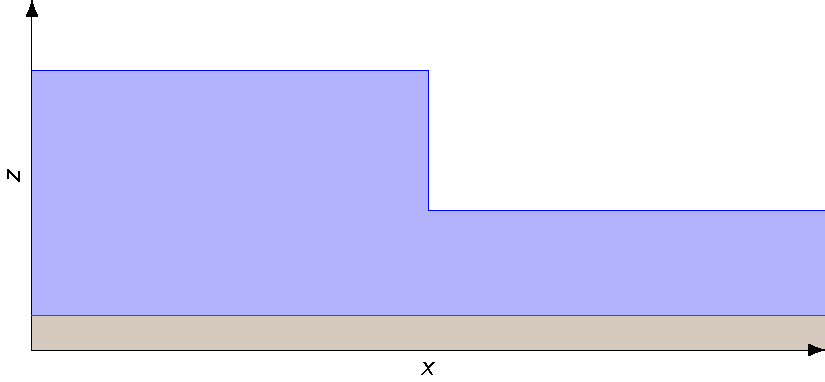
\includegraphics[width=\textwidth]{./Pics/SteepGradients/Wavetank.pdf}
	\end{figure}
\end{frame}	

\begin{frame}{Our New Numerical Solution}
	\begin{figure}
		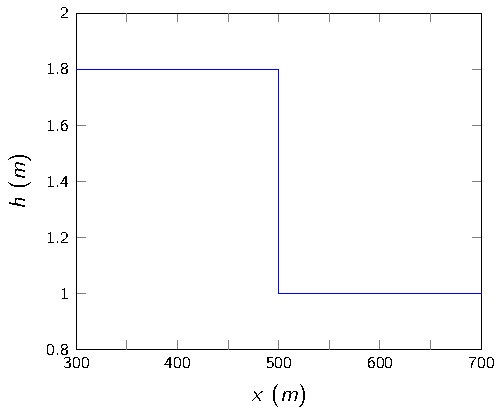
\includegraphics[width=0.5\textwidth]{./Pics/SteepGradients/DBinit.pdf}
		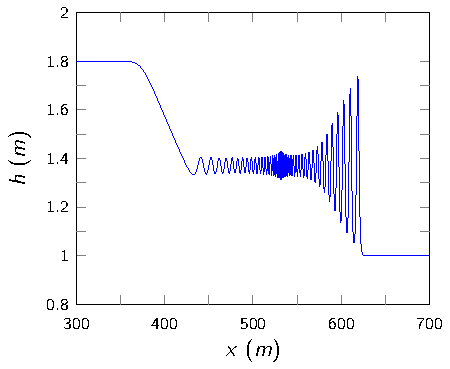
\includegraphics[width=0.5\textwidth]{./Pics/SteepGradients/DBfint.pdf}
	\end{figure}
	\blfootnote{Pitt, J., Zoppou, C., and Roberts, S. (2018).
		Behaviour of the Serre Equations in the Presence of Steep
		Gradients Revisited.
		Wave Motion, 76(1):61–77.}
\end{frame}

%What was known
%Previous Work
%Improvements
\begin{frame}{What was known}
	\begin{itemize}
		\item No analytic solutions
		\item Asymptotic results for step gradient problems as $t \rightarrow \infty$
		\item Some experimental comparisons \footnote{Zoppou, C. (2014).
			Numerical Solution of the One-dimensional and Cylindrical
			Serre Equations for Rapidly Varying Free Surface Flows. PhD thesis, Australian National University.}
		\item Other numerical solutions from the literature; some solving the actual steep gradient problem and some solving a smoothed initial water profile.
		\end{itemize}
\end{frame}

\begin{frame}{Solution}
	\blfootnote{Pitt, J., Zoppou, C., and Roberts, S. (2018).
		Behaviour of the Serre Equations in the Presence of Steep
		Gradients Revisited.
		Wave Motion, 76(1):61–77.}
	\begin{itemize}
		\item Demonstrate convergence to one solution for many numerical methods
		\item Demonstrate good agreement with asymptotic results
		\item Comprehensively review many numerical methods and smoothing techniques from the literature
	\end{itemize}
	
\end{frame}

\begin{frame}{Convergence}
		\begin{figure}
			\includegraphics[width=0.8\textwidth]{./Pics/SteepGradients/dx0/4/1-figure0.pdf}
		\end{figure}
\end{frame}
\begin{frame}
	\begin{figure}
		\includegraphics[width=0.8\textwidth]{./Pics/SteepGradients/dx0/46/1-figure0.pdf}
	\end{figure}
\end{frame}
\begin{frame}
	\begin{figure}
		\includegraphics[width=0.8\textwidth]{./Pics/SteepGradients/dx0/468/1-figure0.pdf}
	\end{figure}
\end{frame}
\begin{frame}
	\begin{figure}
		\includegraphics[width=0.8\textwidth]{./Pics/SteepGradients/dx0/all/1-figure0.pdf}
	\end{figure}
\end{frame}

\begin{frame}{Asymptotic Results}
	\begin{figure}
		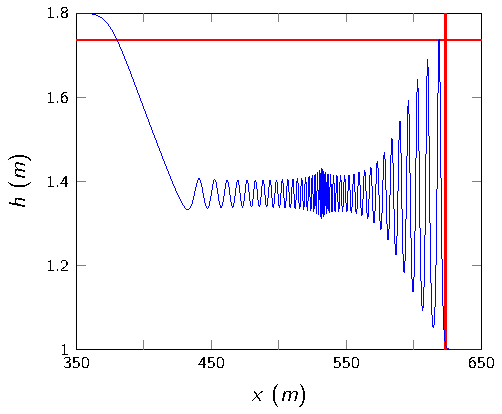
\includegraphics[width=0.8\textwidth]{./Pics/SteepGradients/DSWap1.pdf}
	\end{figure}
\end{frame}

\begin{frame}{Review of Smoothing and Methods}
	\begin{itemize}
		\item Demonstrated that behaviour is consistent across many numerical methods
		\item Were able to explain why the behaviour had not previously been observed
	\end{itemize}
\end{frame}

\begin{frame}{Result}
	Our numerical solutions for the steep gradient problems are well validated \footnote{Pitt, J., Zoppou, C., and Roberts, S. (2018).
		Behaviour of the Serre Equations in the Presence of Steep
		Gradients Revisited.
		Wave Motion, 76(1):61–77.}
\end{frame}

\begin{frame}{Progress}
	\begin{itemize}
		\item[3D:] Extension of the method to 3D flows  \checkmark
		\item[Robust:] Validation of model with steep gradients in free surface \checkmark 
		\item[Robust:] Validation of model in the presence of dry beds 
	\end{itemize}
\end{frame}

\subsection{Solution in the Presence of Dry Beds}
%What was known
%Previous Work
%Improvements
\begin{frame}{Statement of Problem}
	Properly handle interaction of waves and the dry bed
		\begin{figure}
			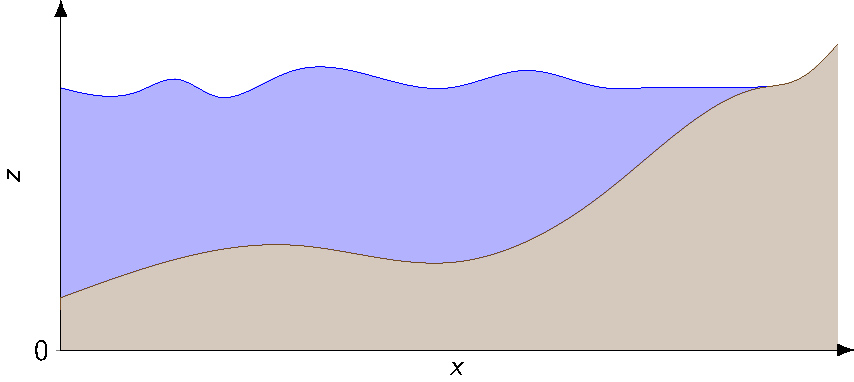
\includegraphics[width=\textwidth]{./Pics/WaterModelDiagrams/FressSurface.pdf}
		\end{figure}
\end{frame}

\begin{frame}{What was known}
	\begin{itemize}
		\item No analytic solutions
		\item A variety of numerical techniques only validated against experimental data
	\end{itemize}
\end{frame}

\begin{frame}{Solution}
	\begin{itemize}
		\item Solved modified equations that did possess analytic solutions
		\item Compared with experimental data
	\end{itemize}
	\begin{figure}
		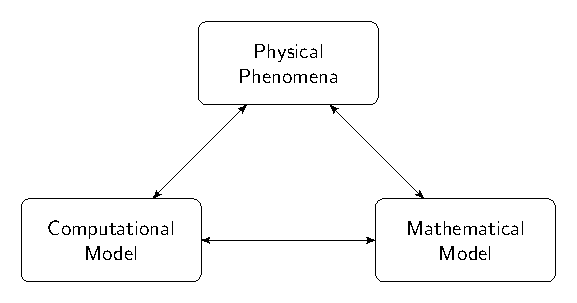
\includegraphics[width=0.8\textwidth]{./Pics/ModelDiagrams/FlowChart.pdf}
	\end{figure}
\end{frame}

\begin{frame}{Constructing Modified Equations}
	\begin{itemize}
		\item Pick functions for height, velocity and bed: $h^*$, $u^*$ and $b^*$
		\item Add Source terms to Serre equations that force a solution for $h^*$, $u^*$ and $b^*$
		\item Validation tests
	\end{itemize}
\end{frame}
\begin{frame}{Pick Functions}

\begin{figure}
	\centering
	\begin{subfigure}{0.5\textwidth}
		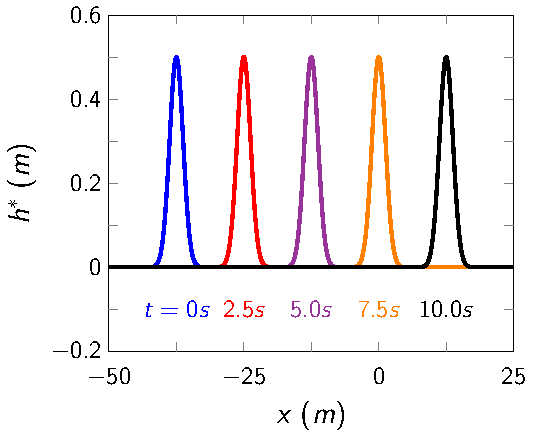
\includegraphics[width=0.8\textwidth]{./Pics/DryBed/Forced/h.pdf}
	\end{subfigure}%
	\begin{subfigure}{0.5\textwidth}
		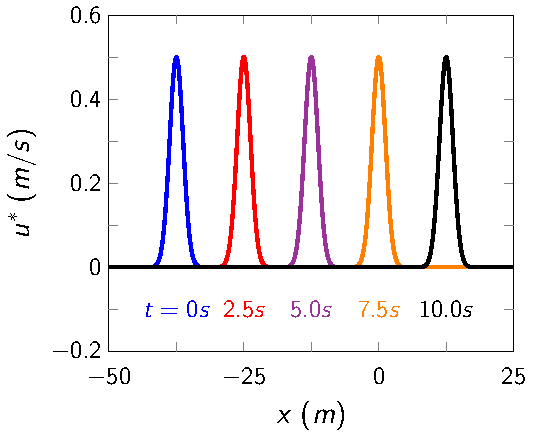
\includegraphics[width=0.8\textwidth]{./Pics/DryBed/Forced/u.pdf}
	\end{subfigure}
	\begin{subfigure}{0.5\textwidth}
		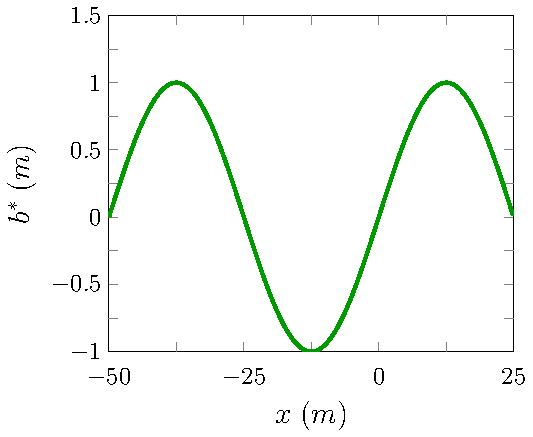
\includegraphics[width=0.8\textwidth]{./Pics/DryBed/Forced/binitial.pdf}
	\end{subfigure}%
	\begin{subfigure}{0.5\textwidth}
		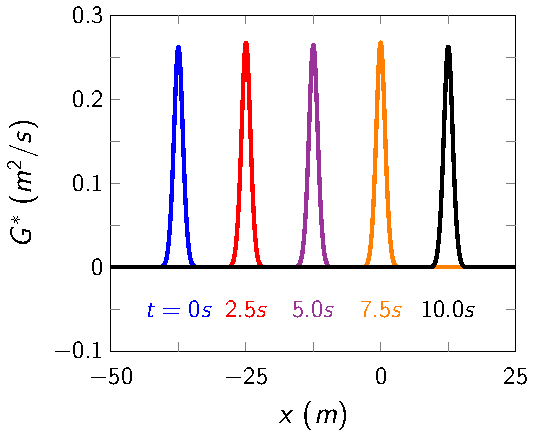
\includegraphics[width=0.8\textwidth]{./Pics/DryBed/Forced/G.pdf}
	\end{subfigure}
\end{figure}
	
\end{frame}

\begin{frame}{Modify Equations}
		\begin{align*}
		& \frac{\partial h}{\partial t} + \dfrac{\partial (uh)}{\partial x} = S_h^* ,  \\ \nonumber \\
		\begin{split}
		\frac{\partial G}{\partial t}  + \frac{\partial}{\partial x} \left( {u} G + \frac{gh^2}{2} - \frac{2}{3}h^3 \left[\frac{\partial {u}}{\partial x}\right]^2 + h^2 {u}\frac{\partial {u}}{\partial x}\frac{\partial b}{\partial x} \right) \\ + \frac{1}{2}h^2 {u} \frac{\partial {u}}{\partial x} \frac{\partial^2 b}{\partial x^2}  - h {u}^2\frac{\partial b}{\partial x}\frac{\partial^2 b}{\partial x^2} + gh\frac{\partial b}{\partial x} = S_G^* .
		\end{split}
		\end{align*}
		$S_h^*$ and $S_G^*$ are just the LHS  with the quantities replaced by their associated chosen function. We solve the LHS using our method and add in the source terms on the RHS analytically.
\end{frame}

\begin{frame}{Results $t=0s$}
\begin{figure}
	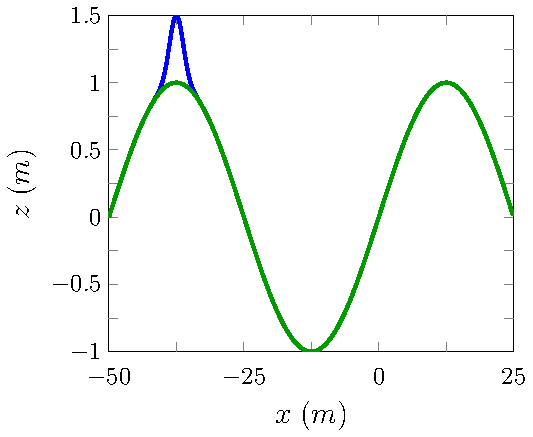
\includegraphics[width=0.8\textwidth]{./Pics/DryBed/Forced/Stages0.pdf}
\end{figure}
\end{frame}

\begin{frame}{Results $t=0s,2.5s$}
	\begin{figure}
		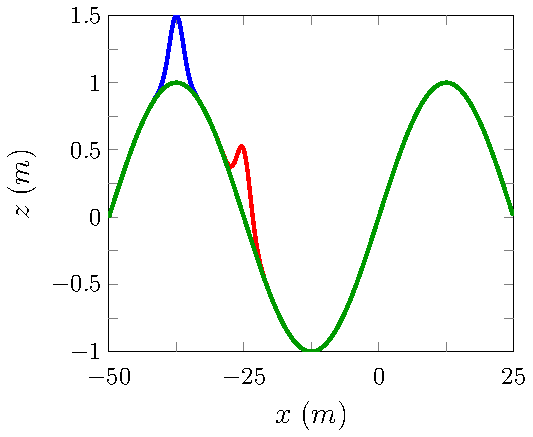
\includegraphics[width=0.8\textwidth]{./Pics/DryBed/Forced/Stages025.pdf}
	\end{figure}
\end{frame}

\begin{frame}{Results $t=0s,2.5s,5.0s$}
	\begin{figure}
		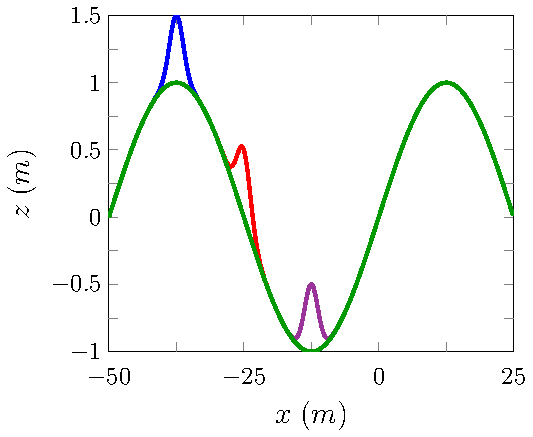
\includegraphics[width=0.8\textwidth]{./Pics/DryBed/Forced/Stages02550.pdf}
	\end{figure}
\end{frame}

\begin{frame}{Results $t=0s,2.5s,5.0s,7.5s$}
	\begin{figure}
		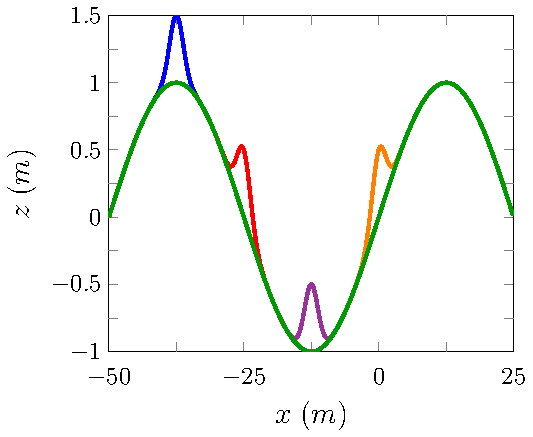
\includegraphics[width=0.8\textwidth]{./Pics/DryBed/Forced/Stages0255075.pdf}
	\end{figure}
\end{frame}

\begin{frame}{Results $t=0s,2.5s,5.0s,7.5s,10.0s$}
	\begin{figure}
		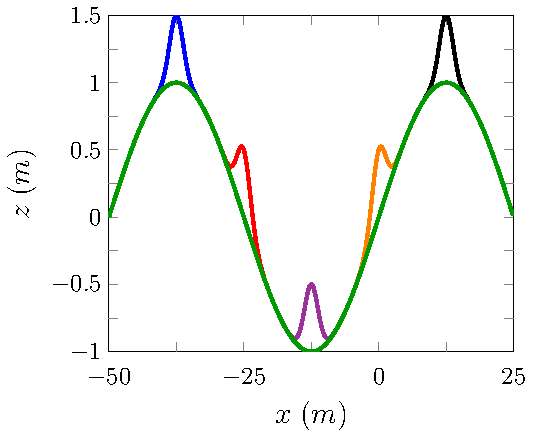
\includegraphics[width=0.8\textwidth]{./Pics/DryBed/Forced/Stages0255075100.pdf}
	\end{figure}
\end{frame}

\begin{frame}{Modified Equations Validation Conclusions}
\begin{itemize}
	\item Very strong test that we are actually solving the Serre equations accurately as all terms must be accurately approximated
	\item Can measure the convergence of numerical solutions to the force solutions
\end{itemize}
\end{frame}

	
\begin{frame}{Experimental Data}
	\begin{figure}
		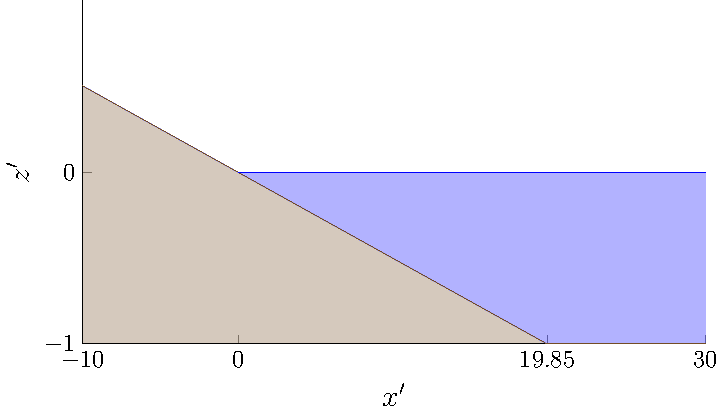
\includegraphics[width=1\textwidth]{./Pics/DryBed/Syn/WavetankArtifical.pdf}
	\end{figure}
\end{frame}

\begin{frame}{$t=30s$}
	\begin{figure}
		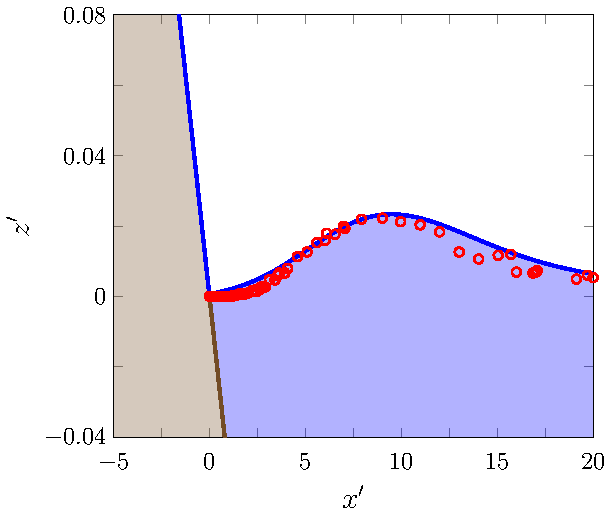
\includegraphics[width=0.8\textwidth]{./Pics/DryBed/Syn/30s.pdf}
	\end{figure}
\end{frame}

\begin{frame}{$t=40s$}
	\begin{figure}
		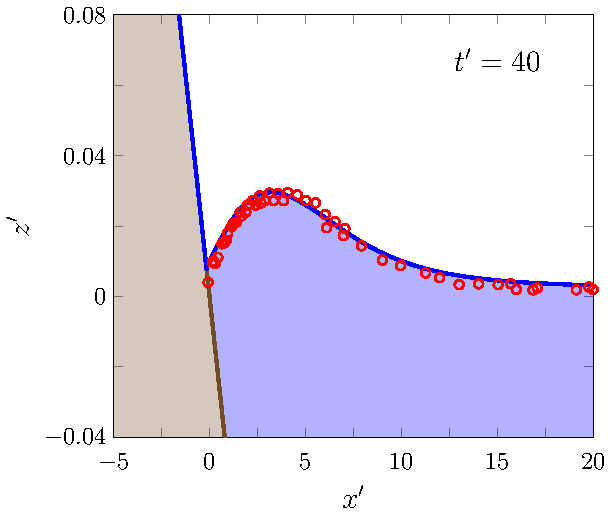
\includegraphics[width=0.8\textwidth]{./Pics/DryBed/Syn/40s.pdf}
	\end{figure}
\end{frame}

\begin{frame}{$t=50s$}
	\begin{figure}
		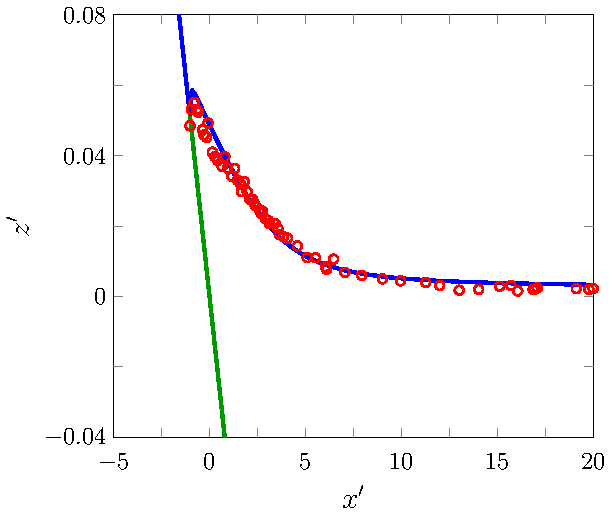
\includegraphics[width=0.8\textwidth]{./Pics/DryBed/Syn/50s.pdf}
	\end{figure}
\end{frame}

\begin{frame}{$t=60s$}
	\begin{figure}
		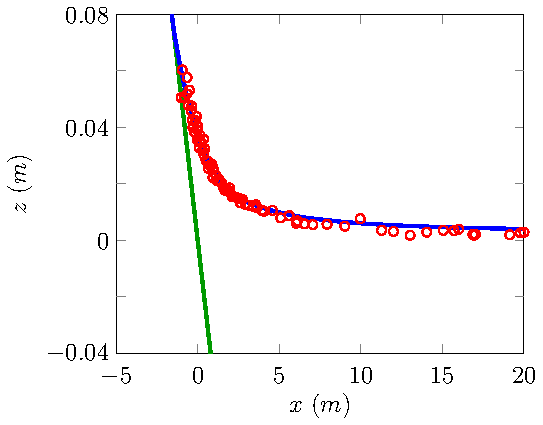
\includegraphics[width=0.8\textwidth]{./Pics/DryBed/Syn/60s.pdf}
	\end{figure}
\end{frame}

\begin{frame}{$t=70s$}
	\begin{figure}
		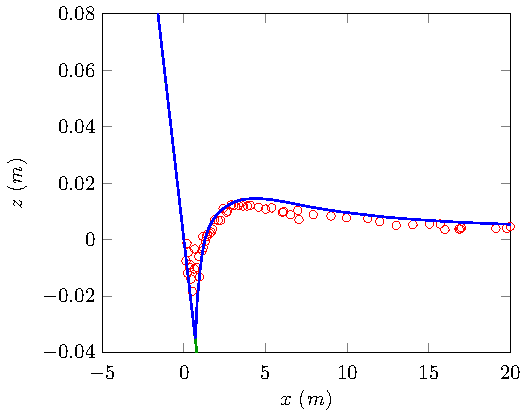
\includegraphics[width=0.8\textwidth]{./Pics/DryBed/Syn/70s.pdf}
	\end{figure}
\end{frame}
\begin{frame}{Experimental Validation Conclusions}
	\begin{itemize}
		\item Demonstrates that our computational model agrees with the physical process
		\item not a very stringent test as there are many source of errors
		\item few experimental results for non breaking waves
	\end{itemize}
\end{frame}

\begin{frame}{Progress}
	\begin{itemize}
		\item[3D:] Extension of the method to 3D flows  \checkmark
		\item[Robust:] Validation of model with steep gradients in free surface \checkmark 
		\item[Robust:] Validation of model in the presence of dry beds \checkmark
	\end{itemize}
\end{frame}

\begin{frame}{Conclusions}
	\begin{itemize}
		\item Developed a Robust Computational Model from the Serre equations for the 2D water wave problem
	\end{itemize}
	\begin{figure}
		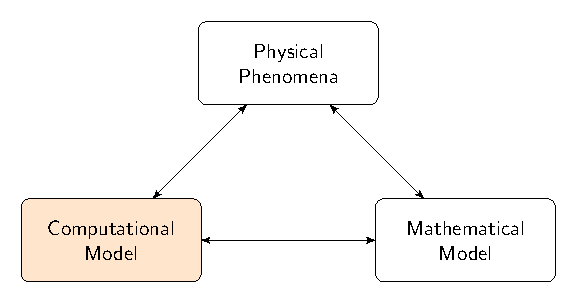
\includegraphics[width=\textwidth]{./Pics/ModelDiagrams/FlowChartHigh3O.pdf}
	\end{figure}
\end{frame}

\begin{frame}[allowframebreaks]
	\frametitle{References}
	\bibliographystyle{apalike}
	\bibliography{bibliography.bib}
\end{frame}

\end{document}